% me=0 student solutions (ps file), me=1 - my solutions (sol file),
% me=2 - assignment (hw file)
\def\me{1} \def\num{4} %homework number

\def\due{11 pm, March 10} %due date

\def\course{APMA 1655 Honors Statistical Inference I} 

% **** INSERT YOUR NAME HERE ****
\def\name{Tanish Makadia}


% **** INSERT NAMES OF YOUR COLLABORATORS HERE, OR JUST PUT N/A ****
\def\collabs{Garv Gaur}

%

\documentclass[11pt]{article}


% ==== Packages ====
\usepackage{amsfonts}
\usepackage{latexsym}
\usepackage{fullpage}
\usepackage{amsmath}
\usepackage{amssymb}
\usepackage{hyperref}
\usepackage{euler}
\usepackage{amsthm}
\usepackage{graphicx}
\usepackage{bbm}
\usepackage{pgfplots}
\usepackage{tikz}

% \setlength{\oddsidemargin}{.0in} \setlength{\evensidemargin}{.0in}
% \setlength{\textwidth}{6.5in} \setlength{\topmargin}{-0.4in}
\setlength{\footskip}{1in} \setlength{\textheight}{8.5in}

\newcommand{\handout}[5]{
\renewcommand{\thepage}{#5, Page \arabic{page}}
  \noindent
  \begin{center}
    \framebox{ \vbox{ \hbox to 5.78in { {\bf \course} \hfill #2 }
        \vspace{4mm} \hbox to 5.78in { {\Large \hfill #5 \hfill} }
        \vspace{2mm} \hbox to 5.78in { {\it #3 \hfill #4} }
       
        \vspace{2mm} \hbox to 5.78in { {\it Collaborators: \collabs
            \hfill} }
           
        \vspace{2mm}
        \begin{itemize}
       
       \item You are strongly encouraged to work in groups, but solutions must be written independently. 

        \end{itemize}
      } }
  \end{center}
  
  \vspace*{4mm}
}


\newcounter{pppp}
\newcommand{\prob}{\arabic{pppp}} %problem number
\newcommand{\increase}{\addtocounter{pppp}{1}} %problem number

% Arguments: Title, Number of Points
\newcommand{\newproblem}[2]{
    \increase
    \section*{Problem \prob~(#1) \hfill {#2}}
}



\def\squarebox#1{\hbox to #1{\hfill\vbox to #1{\vfill}}}
\def\qed{\hspace*{\fill}
  \vbox{\hrule\hbox{\vrule\squarebox{.667em}\vrule}\hrule}}
\newenvironment{solution}{\begin{trivlist}\item[]{\bf Solution:}}
  {\qed \end{trivlist}}
\newenvironment{solsketch}{\begin{trivlist}\item[]{\bf Solution
      Sketch:}} {\qed \end{trivlist}}
\newenvironment{code}{\begin{tabbing}
    12345\=12345\=12345\=12345\=12345\=12345\=12345\=12345\= \kill }
  {\end{tabbing}}

%\newcommand{\eqref}[1]{Equation~(\ref{eq:#1})}

\newcommand{\hint}[1]{({\bf Hint}: {#1})}
% Put more macros here, as needed.
\newcommand{\room}{\medskip\ni}
\newcommand{\brak}[1]{\langle #1 \rangle}
\newcommand{\bit}[1]{\{0,1\}^{#1}}
\newcommand{\zo}{\{0,1\}}
\newcommand{\C}{{\cal C}}
\newcommand{\1}{\mathbbm{1}}
\newcommand{\p}{\mathbb{P}}

\newcommand{\nin}{\not\in}
\newcommand{\set}[1]{\{#1\}}
\renewcommand{\ni}{\noindent}
\renewcommand{\gets}{\leftarrow}
\renewcommand{\to}{\rightarrow}
\newcommand{\assign}{:=}

\newcommand{\AND}{\wedge}
\newcommand{\OR}{\vee}

\newcommand{\For}{\mbox{\bf for }}
\newcommand{\To}{\mbox{\bf to }}
\newcommand{\Do}{\mbox{\bf do }}
\newcommand{\If}{\mbox{\bf if }}
\newcommand{\Then}{\mbox{\bf then }}
\newcommand{\Else}{\mbox{\bf else }}
\newcommand{\While}{\mbox{\bf while }}
\newcommand{\Repeat}{\mbox{\bf repeat }}
\newcommand{\Until}{\mbox{\bf until }}
\newcommand{\Return}{\mbox{\bf return }}
\newcommand{\Halt}{\mbox{\bf halt }}
\newcommand{\Swap}{\mbox{\bf swap }}
\newcommand{\Ex}[2]{\textrm{exchange } #1 \textrm{ with } #2}



\begin{document}

\handout{}{ }{Name: \name{}}{Due: \due}{Homework \num}


\section{Review}

\subsection{Definition of Discrete Random Variables}

Let $(\Omega,\mathbb{P})$ be a probability space. Suppose $X$ is a random variable defined on $\Omega$, and $F_X$ is the CDF of $X$.
    \begin{enumerate}
        \item We say $X$ is a \textbf{discrete random variable} if its CDF $F_X$ is of the following form
        \begin{align}\label{eq: def of discrete CDF}
            \boxed{F_X(x)=\sum_{k=0}^K p_k\cdot\mathbf{1}_{[x_k,\,+\infty)}(x),}
        \end{align}
        where $p_k\ge0$ for all $k=1,2,\ldots,K$ and $\sum_{k=0}^K p_k=1$; the $K$ is allowed to be $\infty$.

        \item If $X$ is a discrete random variable whose CDF is of the form in Eq.~\eqref{eq: def of discrete CDF}, we call the ordered sequence $\{p_k\}_{k=0}^K$ as the \textbf{probability mass function (PMF)}$^\dagger$\footnote{$\dagger$: The ordered sequence $\{p_k\}_{k=0}^K$ is conventionally called as a function. You may view the map $k\mapsto p_k$ as a function. I think the reason $\{p_k\}_{k=0}^K$ is called a function is to make the names ``PMF" and ``PDF" look similar. In addition, if you are comfortable with the concept of vectors, you may view the ordered sequence $\{p_k\}_{k=0}^K$ as a vector $(p_0, p_1,\ldots,p_K)$; if $K=\infty$, this vector is infinitely long.} of $X$. 
    \end{enumerate}

\subsection{Independence between Events}

Let $(\Omega,\mathbb{P})$ be a probability space. Suppose $\Tilde{A}$ and $\Tilde{B}$ are two events. We say $\Tilde{A}$ and $\Tilde{B}$ are \textbf{independent} if $\mathbb{P}(\Tilde{A}\cap \Tilde{B})= \mathbb{P}(\Tilde{A}) \cdot \mathbb{P}(\Tilde{B})$.

\subsection{Independence between Random Variables --- Version I}

Let $Y$ and $Z$ be two random variables defined on the probability space $(\Omega,\mathbb{P})$. We say that $Y$ and $Z$ are independent if they satisfy the following \textbf{for any} subsets $A\subset\mathbb{R}$ and $B\subset\mathbb{R}$
    \begin{align*}
       \boxed{ \mathbb{P}\left(\{\omega\in\Omega \,:\, Y(\omega)\in A \text{ and }Z(\omega)\in B\}\right) = \mathbb{P}\left(\{\omega\in\Omega \,:\, Y(\omega)\in A \}\right) \cdot \mathbb{P}\left(\{\omega\in\Omega \,:\, Z(\omega)\in B\}\right).}
    \end{align*}

\subsection{Independence between Random Variables --- Version II}

Let $Y$ and $Z$ be two random variables defined on the probability space $(\Omega,\mathbb{P})$. We say that $Y$ and $Z$ are independent if the following is true: \textbf{for any} subsets $A\subset \mathbb{R}$ and $B\subset \mathbb{R}$, the following two events are independent
    \begin{align*}
        \Tilde{A}=\{\omega\in\Omega: Y(\omega)\in A\},\ \ \ \ \ \Tilde{B}=\{\omega\in\Omega: Z(\omega)\in B\}.
    \end{align*}

\section{Problem Set}

\begin{enumerate}

\item (2 points) Let $n$ be a positive integer, and $\Omega \overset{\operatorname{def}}{=}\{1,2,\ldots,n\}$. Suppose $\mathbb{P}$ is a function of subsets of $\Omega$ defined as follows
\begin{align*}
\mathbb{P}(A)\overset{\operatorname{def}}{=}\frac{\# A}{\#\Omega}, \ \ \text{ for all }A\subset \Omega.
\end{align*}
We define a random variable $X$ as follows
\begin{align*}
    X(\omega)=\omega,\ \ \ \text{ for all }\omega\in\Omega=\{1,2,\ldots,n\}.
\end{align*}
Suppose you have done the following
\begin{itemize}
    \item You have proved that $(\Omega,\mathbb{P})$ is a probability space (see HW 1).
    \item You have derived the CDF $F_X$ of $X$ (see HW 3).
\end{itemize}

\textbf{Please represent the CDF $F_X$ in the form in Eq.~\eqref{eq: def of discrete CDF}. Specifically, please show what the $K$, $\{p_k\}_{k=0}^K$, and $\{x_k\}_{k=0}^K$ in Eq.~\eqref{eq: def of discrete CDF} should be.}

\begin{align*}
        F_X(x)&=\frac{1}{n}\1_{[1,+\infty)}(x)+\frac{1}{n}\1_{[2,+\infty)}(x)+\cdots + \frac{1}{n}\1_{[n,+\infty)}(x)\\
        &= \sum_{k=0}^{n-1}\frac{1}{n}\cdot \1_{[k+1,+\infty)}(x)
\end{align*}
Therefore, 
\[K=n-1;\ \ \{p_k\}^K_{k=0}=\{\frac{1}{n}\}^{n-1}_{k=0};\ \ \{x_k\}_{k=0}^{n-1}=\{k+1\}^{n-1}_{k=0}\]

\item (2 points) Let $Y$ and $Z$ be random variables defined on the probability space $(\Omega,\mathbb{P})$; the distribution of the random variable $X$ defined as follows
\begin{align}\label{eq: example whose dist is neither conti nor disc}
    \begin{aligned}
    & X(\omega) \overset{\operatorname{def}}{=} Y(\omega)+(1-Y(\omega))\cdot Z(\omega), \ \ \ \text{ for all }\omega\in\Omega,\ \ \mbox{ where} \\
    & Y\sim \operatorname{Bernoulli}\left(\frac{1}{2}\right), \ \ \ \ Z\sim N(0,1), \\
    &\text{$Y$ and $Z$ are independent.}
    \end{aligned}
 \end{align}
Then, we claim that the CDF of the random variable $X$ defined in Eq.~\eqref{eq: example whose dist is neither conti nor disc} is the following
\begin{align}\label{eq: a fair mixture of 1 and N(0,1)}
    \begin{aligned}
        F_X(x) &=\frac{1}{2}\cdot\mathbf{1}_{[1,+\infty)}(x)+ \frac{1}{2}\cdot F_Z(x)\\
    &= \frac{1}{2}\cdot\mathbf{1}_{[1,+\infty)}(x)+ \frac{1}{2}\cdot \int_{-\infty}^x \frac{1}{\sqrt{2\pi}}\cdot e^{-\frac{t^2}{2}} dt,
    \end{aligned}
\end{align}
where $F_X$ denotes the CDF of $X$, and $F_Z$ denotes the CDF of $Z$ (i.e., the CDF of $N(0,1)$). The graph of the CDF in Eq.~\eqref{eq: a fair mixture of 1 and N(0,1)} is presented in Figure \ref{fig: example whose dist is neither conti nor disc}.
\begin{figure}
    \centering
    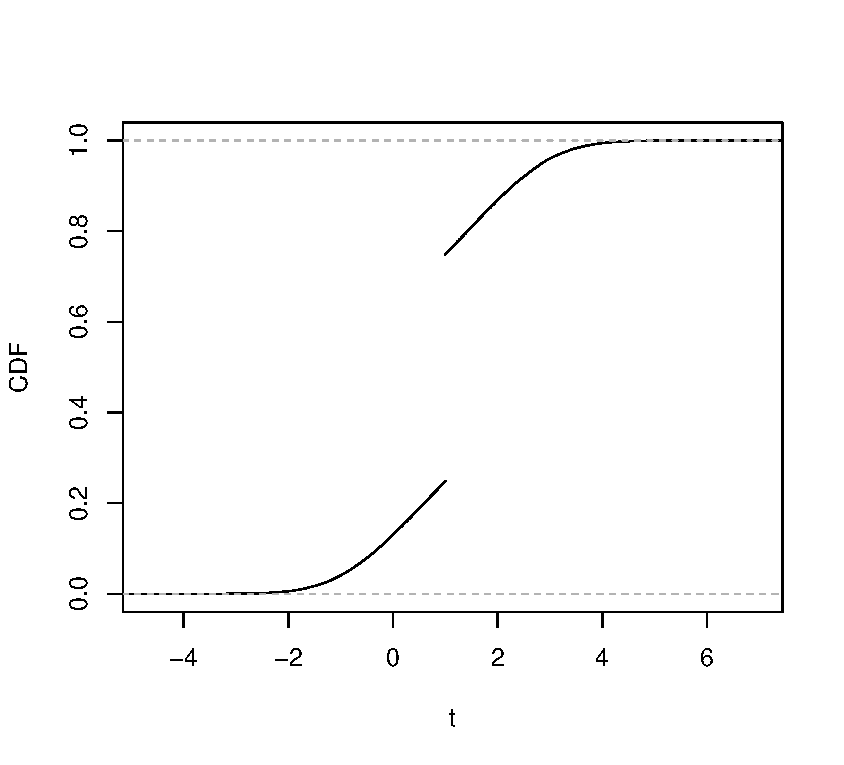
\includegraphics[scale=0.5]{example whose dist is neither conti nor disc.pdf}
    \caption{The CDF of the distribution of $X$ defined in Eq.~\eqref{eq: example whose dist is neither conti nor disc}. This function is neither continuous nor piecewise constant/step-like.}
    \label{fig: example whose dist is neither conti nor disc}
\end{figure}

\textbf{Please prove the formula in Eq.~\eqref{eq: a fair mixture of 1 and N(0,1)}.}

\begin{proof}
    By the law of total probability, 
    \[F_X(x)=\p(X\leq x)=\p(X\leq x\mid Y=1)\cdot \p(Y=1)+\p(X\leq x\mid Y=0)\cdot \p(Y=0)\]
    We will now compute each half of the sum.
    \begin{align*}
        \p(X\leq x\mid Y=1)\cdot \p(Y=1) &= \p(Y+(1-Y)Z\leq x\mid Y=1)\cdot \p(Y=1)\\
        &= \p(1+(1-1)Z\leq x)\cdot \p(Y=1)\\
        &= \p(1\leq x)\cdot \p(Y=1)\\
        &= \frac{1}{2}\1_{[1,+\infty)}(x)
    \end{align*}
    \begin{align*}
        \p(X\leq x\mid Y=0)\cdot \p(Y=0) &= \p(Y+(1-Y)Z\leq x\mid Y=0)\cdot \p(Y=0)\\
        &= \p(0+(1-0)Z\leq x)\cdot \p(Y=0)\\
        &= \p(Z\leq x)\cdot \p(Y=0)\\
        &= \frac{1}{2}F_Z(x)
    \end{align*}
    Therefore, \(F_X(x)=\frac{1}{2}\1_{[1,+\infty)}(x)+\frac{1}{2}F_Z(x)\).
\end{proof}

\item (2 points) Let $Y$, $Z$, and $W$ be random variables defined on the probability space $(\Omega,\mathbb{P})$. Suppose
    \begin{itemize}
        \item $Y\sim\operatorname{Bernoulli}(p)$;
        \item the CDFs of $Z$ and $W$ are $F_Z$ and $F_W$, respectively;
        \item $Y$, $Z$, and $W$ are mutually independent, i.e., $Y$ and $Z$ are independent, $Y$ and $W$ are independent, $Z$ and $W$ are independent.
    \end{itemize} 
    We define a new random variable $X$ by $X(\omega)\overset{\operatorname{def}}{=} Y(\omega)\cdot Z(\omega) + (1-Y(\omega))\cdot W(\omega)$ for all $\omega\in\Omega$. \textbf{Please prove that the CDF of $X$ is the following}
    \begin{align*}
        F_X(x) = p\cdot F_Z(x)+(1-p)\cdot F_W(x).
    \end{align*}

\begin{proof}
    By the law of total probability,
    \[F_X(x)=\p(X\leq x\mid Y=1)\cdot \p(Y=1)+\p(X\leq x\mid Y=0)\cdot \p(Y=0)\]
    We will now compute each half of the sum.
    \begin{align*}
        \p(X\leq x\mid Y=1)\cdot \p(Y=1) &= \p(YZ+(1-Y)W\leq x\mid Y=1)\cdot \p(Y=1)\\
        &= \p(1\cdot Z+(1-1)W\leq x)\cdot \p(Y=1)\\
        &= \p(Z\leq x)\cdot \p(Y=1)\\
        &= p\cdot F_Z(x)
    \end{align*}
    \begin{align*}
        \p(X\leq x\mid Y=0)\cdot \p(Y=0) &= \p(YZ+(1-Y)W\leq x\mid Y=0)\cdot \p(Y=0)\\
        &= \p(0\cdot Z+(1-0)W\leq x)\cdot \p(Y=0)\\
        &= \p(W\leq x)\cdot \p(Y=0)\\
        &= (1-p)\cdot F_W(x)
    \end{align*}
    Together, we have \(F_X(x)=p\cdot F_Z(x)+(1-p)\cdot F_W(x)\).
\end{proof}

\item (2 points) Let $Y$, $Z$, and $W$ be random variables defined on the probability space $(\Omega,\mathbb{P})$. Suppose
    \begin{itemize}
        \item $Y\sim\operatorname{Bernoulli}(1/3)$;
        \item $Z\sim \operatorname{Pois}(1)$;
        \item $W\sim N(0,1)$;
        \item $Y$, $Z$, and $W$ are mutually independent, i.e., $Y$ and $Z$ are independent, $Y$ and $W$ are independent, $Z$ and $W$ are independent.
    \end{itemize} 
    We define a new random variable $X$ by $X(\omega)\overset{\operatorname{def}}{=} Y(\omega)\cdot Z(\omega) + (1-Y(\omega))\cdot W(\omega)$ for all $\omega\in\Omega$. Let $F_X$ denote the CDF of $X$. \textbf{Please draw the graph of $F_X(x)$ for $-1\le x\le 5.5$, i.e., }
    \begin{align*}
        \left\{\left(x, F_X(x)\right) \,:\, -1\le x\le 5.5\right\}.
    \end{align*}

    We have already shown that \(F_X(x)=p\cdot F_Z(x)+(1-p)\cdot F_W(x)\). 
    
    Since \(Y\sim Bernoulli(1/3)\), we have that
    \[p=\p(Y=1)=1/3 \text{ and } 1-p=\p(Y=0)=2/3\]
    Additionally, since \(X\sim Pois(1)\), we have that
    \begin{align*}
        F_Z(x)&=\sum_{k=0}^{+\infty}\frac{1}{ek!}\cdot\1_{[k,+\infty)}(x)\\
        &= \sum_{k=0}^{x}\frac{1}{ek!}
    \end{align*} 
    Finally, since \(W\sim N(0,1)\), we have that 
    \[F_W(x)=\int_{-\infty}^x \frac{1}{\sqrt{2\pi}}\cdot e^{-\frac{1}{2}t^2}dt\]
    Together, 
    \[F_X(x)=\frac{1}{3}\cdot \sum_{k=0}^{x}\frac{1}{ek!} + \frac{2}{3}\cdot\int_{-\infty}^x \frac{1}{\sqrt{2\pi}}\cdot e^{-\frac{1}{2}t^2}dt\]
    The following is the graph of \(F_X(x)\):

    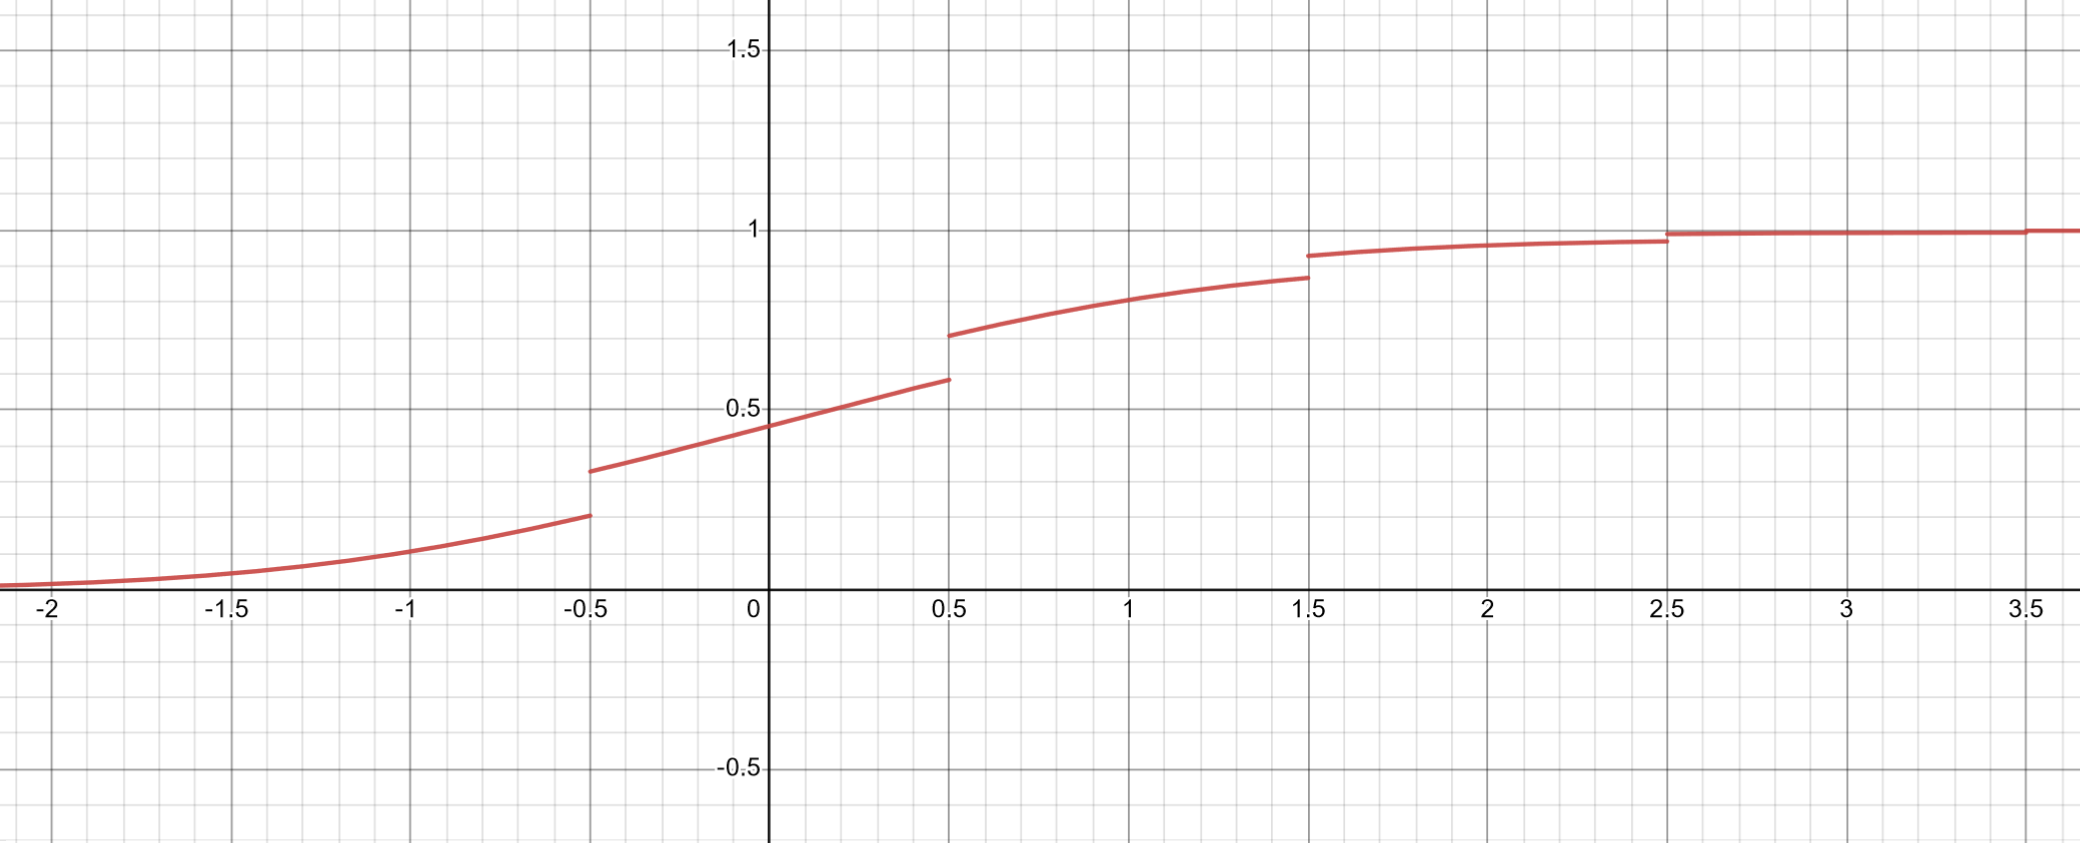
\includegraphics[scale=0.5]{Graph.png}

    \item (2 points) Let $p_{k}=\frac{\lambda^{k} e^{-\lambda}}{k!}$ for all $k=0,1,2,\ldots$, where $k!$ denotes the \href{https://en.wikipedia.org/wiki/Factorial}{factorial} of $k$; conventionally, $0!=1$ (see \href{https://en.wikipedia.org/wiki/Factorial}{Wikipedia}). \textbf{Please prove the following identity}
    \begin{align}\label{eq: expected value of Pois(l) is l}
        \sum_{k=0}^\infty k\cdot p_k=\lambda.
    \end{align}
    \textbf{Remark:} Eq.~\eqref{eq: expected value of Pois(l) is l} shows that the ``expected value" of $\operatorname{Pois}(\lambda)$. We will discuss the concept of expected values in Chapter 3 of my lecture notes.

\begin{proof}
    Since \(p_k=\frac{\lambda^{k} e^{-\lambda}}{k!}\), we have that
    \begin{align*}
        \sum_{k=0}^\infty k\cdot p_k &= \sum_{k=0}^{\infty}k\cdot \frac{\lambda^ke^{-\lambda}}{k!}\\
        &= 0 + \sum_{k=1}^{\infty}k\cdot \frac{\lambda^ke^{-\lambda}}{k!}\\
        &= e^{-\lambda}\sum_{k=1}^{\infty}k\cdot\frac{\lambda^k}{k!}\\
        &= e^{-\lambda}\sum_{k=1}^{\infty}\frac{\lambda^k}{(k-1)!}\\
        &= e^{-\lambda}\sum_{k=1}^{\infty}\frac{\lambda^{k-1}\lambda}{(k-1)!}\\
        &= \lambda\cdot e^{-\lambda}\sum_{k=1}^{\infty}\frac{\lambda^{k-1}}{(k-1)!}\\
        &= \lambda\cdot e^{-\lambda}\sum_{k=0}^{\infty}\frac{\lambda^{k}}{k!}\\
        &= \lambda\cdot e^{-\lambda}\cdot e^\lambda\\
        &= \lambda
    \end{align*}
\end{proof}

\end{enumerate}


\newpage



\end{document}